\chapter{Hardware and Software}\label{ch:hardware_software}

For a long time, people have desired or imagined machines that can compute. Why did it take so long for computers to be invented? Part of the reason is that digital electronics are a relatively recent innovation, building on an understanding of the physics of materials which only came to fruition in the 20\textsuperscript{th} century. However, perhaps a more overarching difficulty is that ``machines that can compute'' is a rather poorly defined idea. What does it mean to compute?

For instance, imagine a 19\textsuperscript{th} century engineer trying to build a computer out of mechanical parts. First he might desire a machine which can add very large numbers. He spends weeks at the drawing board, sketching out a massive contraption with marbles representing digits, funnels to combine digits, gears and pulleys driving dumbwaiters which can physically ``carry the 1,'' and so on. When used just so, it can add up to five-digit numbers. Our engineer thinks he might be able to get up to eight-digit numbers with some more funding, so he presents his prototype to Queen Victoria.

``Fabulous!'' she exclaims. ``Now show me multiplication!'' Our engineer is taken aback. ``Well, your majesty, you see -- this is an adding machine. It does not multiply.'' Victoria's smile quickly fades. ``Oh. Very well then. It does not multiply. What else can it do? Could you extract the third root of 47? Sort a list of a million 32-bit integers? Compute the shortest path between two vertices on a graph?'' For Victoria was a very forward-thinking queen.

``No, your majesty -- I'm afraid this is only an \emph{adding machine}. Perhaps with a royal grant I could build many large contraptions, one for each of the tasks you have set before me.'' Victoria now wears a distinct frown. ``Goodness me,'' she exclaims. ``That just won't do. Imagine all the different computational tasks one might like to carry out. My coffers are not without bound. I cannot fund them all. It is true that separate mechanical tasks require separate machines -- I am perfectly willing to give one grant for the design of a tractor, and another for a pencil sharpener. But a \emph{computer} should \emph{compute}, in some universal sense. I shall not waste my time with adding machines and multiplying machines and root-finding machines and a thousand other such knick-knacks.''

Queen Victoria's suggestion is prescient: one might imagine a machine which can be configured to perform any sort of computational task. In the 1930's, Alan Turing laid the foundations for computer science by giving a mathematical description of just such a machine. With nothing but memory and a simple CPU, it can be set up to read instructions from its memory, and then proceed to follow these instructions, manipulating subsequent data in whatever way was specified. This machine is known today as the \emph{universal Turing machine}.

The actual computers we have today are more complicated than the universal Turing machine, but they exhibit the same fundamental split. The \emph{hardware} -- that is, the bare metal that makes up the physical computer and its associated devices -- is capable of performing any kind of computation. It is left to programmers to create \emph{software} which tells the hardware exactly what computations to carry out. By using different software, the same hardware can perform all of Queen Victoria's tasks, and a great deal more.

In this chapter, we will give a general overview of the many layers that allow software to run, starting with their programs at the top and ending with the hardware at the bottom. This is the first example you will see of a layered architecture; examples of the layers we will discuss are shown in Figure \ref{fig:hw_sw:layers}. We will see a similar structure in the following chapters when we discuss networks. In each case, remember that although all layers are important to understand, as a programmer you will interact mostly with the top layers.

\begin{figure}
    \centering
    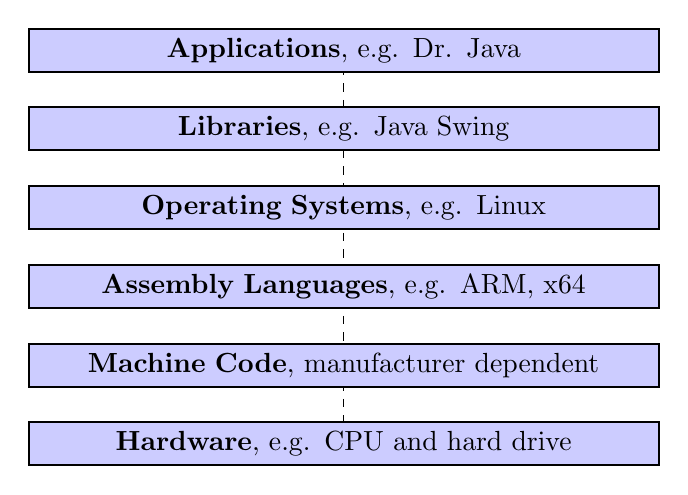
\begin{tikzpicture}[layer/.style={fill=blue!20,minimum width=8cm,align=center,text width=7.5cm,draw=black,solid,line width=.25mm}]
        \draw[dashed,-latex] (0, 4) node[layer] {\textbf{Applications}, e.g. Dr. Java} --
        (0, 3) node[layer] {\textbf{Libraries}, e.g. Java Swing} --
        (0, 2) node[layer] {\textbf{Operating Systems}, e.g. Linux} --
        (0,1) node[layer] {\textbf{Assembly Languages}, e.g. ARM, x64} --
        (0,0) node[layer] {\textbf{Machine Code}, manufacturer dependent} --
        (0, -1) node[layer] {\textbf{Hardware}, e.g. CPU and hard drive};
    \end{tikzpicture}
    \caption{An application such as Dr. Java relies on many layers below, ending with hardware at the bottom.}
    \label{fig:hw_sw:layers}
\end{figure}

\section{Applications}

When you use a computer, you run various applications with perform tasks for you. A computer user might use a web browser to view pages on the Web, a word processor to make flyers, an email client to send messages, a Minesweeper game to kill some time -- all before lunch. Each of these is a separate application, designed by one or more programmers. Dr. Java is also an application.

In the early days of computing, applications were built from the ground up. In fact, one of the earliest ``applications,'' designed in part by Alan Turing himself, was used to break German codes during World War II. This application ran on a computer that was the first of its kind, and so every single detail had to be specified, from such high-level tasks as the mathematical cryptanalysis used to break the codes, all the way down to low-level tasks such as delivering output to the user.

Today, there are systems in place that enable programmers to create new and exciting applications without having to repeat all of the mundane parts that all applications share. Many of these more mundane parts are provided by libraries.

\section{Libraries}

Dr. Java was written using Java itself. The programmers wanted to make an application that could edit and run Java programs. But in order to do this, they need to have a way to display an editable text box containing your code, a way to display your files and let you select one to open, and so on. None of these features was programmed by hand for Dr. Java. Instead, the Dr. Java programmers made use of \emph{libraries}, code which performs common functions and which is made available for any programmer to use. Dr. Java in particular uses a library called Swing, which provides tools for programmers to develop graphical user interfaces (GUIs) using Java.

Libraries are a key component of just about any program. Different libraries may be useful in different contexts. For example, programmers designing websites need libraries which can understand how to determine the current time for users across different timezones, or libraries that understand how to securely store passwords in a database. Programmers designing artificial intelligence systems need libraries which can run digital brains known as artificial neural networks. These libraries are all provided so that nobody has to reinvent the wheel, and programmers can spend their time developing new and exciting applications.

\section{Operating Systems}

Computers today run many different applications, often all at the same time. You might run Dr. Java while using a web browser to read the Java docs and a file explorer to find where you saved your program. Each of these applications wants to use the CPU to run, access the hard drive to view files, display graphics on the screen, and listen for keystrokes from the keyboard. How does the computer manage to balance the needs of all these applications?

This is the job of an \emph{operating system}. The operating system is a special piece of software on a computer which serves as the bedrock for all other software. It is responsible for allocating resources such as CPU time and hard drive access among various applications, managing low-level functionality such as drawing graphics on the screen, and so on. In this class we are using a version of the Linux operating system, which you will learn more about in the next chapter. Other popular operating systems include Microsoft's Windows and Apple's OS X.

\section{BIOS}

Today, it is very likely that the first software loaded onto any computing device is firmware. Firmware is software that helps facilitate other software interacting with the computer device. One notable piece of firmware is called the BIOS (Basic Input/Output System). You would be hard-pressed to find any personal computer or smartphone that doesn't have a BIOS already pre-installed by the device's manufacturer. A BIOS helps facilitate initial loading of programs onto a computer. A BIOS will tell the computer to look for a connected device trying to communicate with the computer (e.g. CD or USB drives). 

\begin{figure}
    \centering
    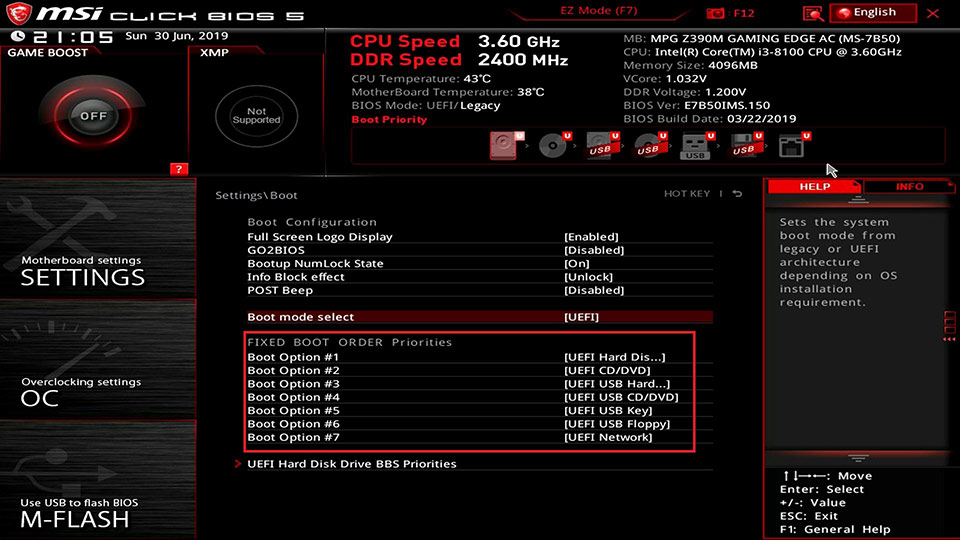
\includegraphics[width=12cm]{images/bios.jpg}
    \caption{Layers of software built up from hardware. Each providing more abstractions and functionality for higher levels to use.}
    \label{fig:hw_sw:bios}
\end{figure}

Figure \ref{fig:hw_sw:bios} shows a relatively modern and user-friendly BIOS interface, with the settings for boot order highlighted. In this instance, the BIOS is set to first boot from an operating system on the hard disk, if one is available. This is the typical scenario for a computer which has already been set up. If there is no operating system on the hard disk, the BIOS is configured to try to boot from a CD or a USB drive instead. These devices might be used to initially install the operating system.

\section{Hardware}

Hardware is the collection of physical devices that make up a computer. The hardware performs the actual computations by manipulating electrical currents. Today most computers are digital, meaning that the computer works by representing data with electrical currents at a high or low voltage. We think of these high-voltages as ones and low-voltages as zeroes. The only thing the hardware understands are these voltages. Different sequences of voltages represent different instructions to the machine. This translation between voltages, or the corresponding binary numbers, and instructions is called the computer's machine language. Not all computers recognize the same machine language. The same sequence of ones and zeroes may not represent the same information on two computers, and it is often manufacturer dependent.

In order to make it easier to write software for their computers, manufacturers will provide another language called assembly language. Typically the assembly language is one of a few popular choices. Most processors today recognize the ARM or the Intel x64 assembly languages. Assembly language is more human-readable than machine code. For example, ARM provides the instruction \ic{ADD} for adding values, and \ic{ADD r3, r1, r2} is a line of assembly language meaning add the values of \ic{r1} and \ic{r2} and store the result in \ic{r3}. The machine code equivalent would be some string of ones and zeroes.

Even though assembly language is a bit easier to understand than machine code, human programmers couldn't get very far if they had to write in assembly language. This is why we have programming languages and compilers. Languages like Java, C++ and others are designed to be relatively straightforward for humans to understand. This way, programmers can specify what they want a program to do in a way that makes sense to them. When the programmer presses compile, a compiler translates the programmer's code into assembly language. The compiler is sort of like a robot programmer: it knows how to read a program in a language like Java, and it understands it as a very precise description of a program that it should write in assembly language. 

\section{Java Virtual Machine}

For a long time, the model we have discussed so far worked well. A program written in an old language, such as C, would be compiled. The compiler would translate the programmer's C code into assembly language, and then the assembly code could be run on the programmer's computer. If the programmer wanted the program to run on a computer with a different assembly language, they could compile their program with a compiler written for that assembly language, and distribute that version of the compiled code accordingly.

This changed when the Internet was created. Suddenly, instead of sending floppy disks or CD-ROMs in the mail to specific intended users, it became possible -- in principle -- to distribute a program broadly by making it available on the Internet. However, since the end user could be using a computer which understands one of many possible assembly languages, the programmer would have to make many different versions of the program available. Even if the programmer could compile her program for every possible assembly language, the user would have to know which version to download, which could be difficult.

Java was created largely to address this issue. When you compile a Java program, you get a \ic{.class} file, which cannot be executed directly by your computer. Instead, you run \ic{java MyClass.class}, which loads a program called the Java Virtual Machine, or JVM. The JVM essentially simulates a computer with a fixed assembly language. When you downloaded the Java Development Kit, part of it was a tool called the Java Runtime Environment which operates the JVM. This way, there is only one way to compile a Java program: you run \ic{javac} and produce a \ic{.class} file. You could put this \ic{.class} file on the Internet, and another Java user could download it and run it on their JVM. The only computer-specific software is the JVM itself, which is available for any kind of computer.

\exercisesection

\begin{exercise}
    Explain why it is important to separate hardware from software.
\end{exercise}

\begin{exercise}
    For each of the following tasks, say which aspect of a computer or a program carries them out.
    \begin{itemize}
        \item Translate programmer's code into assembly language.
        \item Allocate CPU time to different applications.
        \item Provide reusable code to programmers.
        \item Carry out instructions specified by sequences of voltages.
        \item Look for bootable media to assist with installing an operating system.
    \end{itemize}
\end{exercise}

\begin{exercise}
    If assembly languages didn't exist, and hardware only understood their machine code, there would have to be more different versions of which kind of software?
\end{exercise}

\begin{exercise}
    When you compile a Java program, what kind of file do you get? What software is used to run this file?
\end{exercise}